% §3 Axioms --- blueprint chapter 3 (blueprint/src/parts/03-axioms.tex), statements and proofs
% of record verbatim. Drafted 2026-09-11.
%
% Contents and departures from the blueprint chapter:
%   - all three statement nodes transcribed (def:cascade-family, prop:two-members,
%     prop:no-positivity-no-classification) under their markers; the two propositions are
%     `notready` in the blueprint and the prose says exactly what is unchecked in each: the
%     density sentence of the Matérn member (cited, §10) and the Wiener-algebra construction of
%     h_{s,t} (priced, not attempted) --- the section's frontier, named and not hidden;
%   - a short motivation of the axiom list precedes the definition (paper-only; Paper I's axioms
%     section motivates each axiom at length, and this article's introduction carries the series
%     map, so a paragraph per group of axioms is what is added here);
%   - rem:provenance-pauwels and rem:signed-levy-uniqueness are copied; rem:provenance-causal is
%     copied as this section's one relation-to-the-causal-theory remark, its last sentence
%     reworded now that every section carries such a remark; the draft's Remark 3.4 (the
%     section map) is dropped, per the outline's decision;
%   - the blueprint's chapter references become section references.
% Forward references resolved for v0.1 (2026-09-12): prop:matern-exponent is Appendix A; the
% density identification (prop:matern-density, chapter 10, not transcribed) is a cited closed
% form here, A15's anchors; the moment clause is Lean core since R156 (2026-09-14, the density
% sentence dropped from the statement); the extreme-ray claim points at rem:gaussian-extreme
% in §7 instead of chapter 8's prop:choquet-cone; the section pointers to chapters 9-10 are gone.

\section{Spatial measurement: the axioms}\label{sec:axioms}

This section assembles the axiom system of the paper: a list of requirements on the
measurement of a signal on the line, each motivated in turn and collected in
Definition~\ref{def:cascade-family}. The substantive change from
\sscite{pauwels1995extended} is one axiom, the cascade property of
\S\ref{sec:axioms-cascade}, and it is the subject of the paper. The smaller differences are
recorded in Remark~\ref{rem:provenance-pauwels}. Positivity is stated in its place in the
list, but the section is arranged so that its role stays visible:
\S\ref{sec:axioms-nopositivity} says what the other axioms admit without it, and
\S\ref{sec:characterization} what it cuts that down to.

It is impossible to measure the value of a signal at a point: a measurement collects input
from a region of nonvanishing extent, an \emph{extended point} \sscite{florack1997image}.
What an observer holds is therefore a record of the signal at some resolution, never the
signal itself, and a multi-scale front end maintains a family of such records, indexed by a
scale. The front end is \emph{uncommitted}: it is built before anything is known about what
the signals will contain, so the family of records cannot be derived from a signal model
and must be derived from requirements on the measurement process itself. Those
requirements are what this section states.

The requirements are those of Pauwels, Van Gool, Fiddelaers and Moons
\sscite{pauwels1995extended}, restated for operators indexed by pairs of scales, and each
is motivated in turn below. Space has no arrow: an observer may look both ways, and a record
may be reread. So no causality requirement arises, and the symmetry that does, reflection,
is stated in \S\ref{sec:axioms-symmetry}.

A spatial measurement is an operator that smooths the signal. Signals are integrable,
$\Lone = L^1(\RR, dx)$, with positive cone $L^1_+$ and $\int f := \int_\RR f(x)\,dx$. This
and the other notation used informally here is fixed in \S\ref{sec:preliminaries}. Because
a record is itself a signal, and is measured further in the cascade of
\S\ref{sec:axioms-cascade}, the measurement operators are indexed by ordered pairs of
scales,
\[
  \Phis{s}{t} : \Lone \to \Lone, \qquad 0 \le s \le t < \infty,
\]
with $\Phis{s}{t}$ carrying the record at scale $s$ to the record at the coarser scale $t$,
and the signal itself as the record at scale $0$. In the classical theory a single scale
index suffices. Why two are needed here is the point of \S\ref{sec:axioms-cascade}. The
apertures (the measures realizing these operators) are not postulated: that the
operators are convolutions is recovered from the axioms in \S\ref{sec:representation}, and
which convolutions in \S\ref{sec:characterization}.

The formal theory is set on the closed half-line $[0,\infty)$ of scales, with the signal as
the record at scale $0$ and $\Phis{t}{t} = \mathrm{Id}$ on the diagonal. Neither is a
realizable measurement. Both enter as the limits the continuity requirement of
\S\ref{sec:axioms-continuity} refers to, as the Dirac measure enters the extended-point
axiom of the classical theory, $\phi_t \to \delta$ as $t \to 0$: as a limit the family
approaches and never attains. Nothing is measured \emph{at} scale $0$. Every statement
below is about the family and its limits.

\subsection{Linearity, positivity, and mass}\label{sec:axioms-linearity}

An uncommitted front end treats all intensity levels alike and prefers no signal feature
over another. Superposition is the operational form of that indifference: a device that
does not respect it responds to some combinations of inputs differently from the sum of
its responses, and has thereby singled those combinations out before anything is known
about the signals. So each $\Phis{s}{t}$ is linear. This is the assumption on which the
convolution route of \S\ref{sec:representation} rests. The nonlinear scale-space
axiomatics \sscite{alvarez1993axioms}, which give it up, are a different theory. Measurement
is also stable (a small signal leaves a small record), which on $\Lone$ is boundedness
of each $\Phis{s}{t}$ (A1).

An intensity signal is nonnegative, and a measurement of nonnegative input that reports
negative values has created structure of its own, structure of the apparatus rather
than of the signal. Measurement preserves the positive cone (A4). This is the axiom whose
role the paper singles out (\S\ref{sec:axioms-nopositivity}, \S\ref{sec:characterization}).

Smoothing an image may not change its average intensity (\emph{gray-level invariance}),
so the smoothing operator is conservative: it redistributes mass and neither creates
nor absorbs any. On integrable signals the invariant quantity is the total mass $\int f$,
and this is (A5). A device that loses mass models absorption rather than measurement, and
is not pursued.

\subsection{Symmetry: translation and reflection}\label{sec:axioms-symmetry}

A front end built before its signals has no preferred position and no preferred
direction on the line.

No preferred position: each $\Phis{s}{t}$ commutes with the translations
$(\Tr{a}f)(x) = f(x - a)$, $a \in \RR$, which is (A2).

No preferred direction: each $\Phis{s}{t}$ commutes with the reflection $(Rf)(x) = f(-x)$,
which is (A3). Pauwels et al.\ impose it as evenness of the kernel. Stated on the operator
it is a symmetry, and it acts in two directions at once. It admits the even apertures, the
Gaussian among them, and it excludes every one-sided aperture and every aperture whose
centre is displaced from the origin, that is any net drift of the records across scale. The
one aperture that (A3) admits and that measures nothing, the identity, is removed by (ND)
below. So the class has no degenerate member, and its boundary member is the Gaussian
itself (\S\ref{sec:characterization}).

\subsection{Covariance}\label{sec:axioms-covariance}

A front end built before its signals has no preferred unit of length either: rescaling
the line must carry the family into itself. The mass-preserving dilations are
\[
  (\Dil{\lambda}f)(x) = \lambda^{-1}f(x/\lambda), \qquad \lambda > 0 .
\]
One point requires care before the requirement can be stated. Nothing so far ties the scale
index $t$ to a unit of length: the scale axis is, at this stage, only an ordered
parametrization of the records (which is finer, which is coarser), and the labels
themselves have no metric meaning. A rescaling of the line can therefore not be asked to
fix each operator. It can only be asked to map the family onto itself, with the scale
labels rearranged. Formally: there is a family $(S_\lambda)_{\lambda > 0}$ of increasing
bijections of $[0,\infty)$ with
\[
  \Dil{\lambda}\,\Phis{s}{t} \;=\; \Phi_{S_\lambda s,\,S_\lambda t}\,\Dil{\lambda}
  \qquad \text{for all } 0 \le s \le t,\ \lambda > 0,
\]
which is (A8) (Figure~\ref{fig:covariance-square}). The axioms, with the nondegeneracy of
\S\ref{sec:axioms-continuity}, determine each $S_\lambda$ uniquely, and
\S\ref{sec:covariance} recovers a canonical scale parametrization from the action. This is
the free rescaling function of \sscite{pauwels1995extended}, and the difference is only
where it enters: posited there as part of the kernel's form, it is here recovered from a
covariance requirement in which it is left free. The requirement is \emph{full} covariance, every
$\lambda > 0$. The discrete form, $\lambda \in \beta^{\ZZ}$ for a fixed ratio $\beta$ between
successive scales, is a weaker requirement with a theory of its own, and it is
outside this paper.

% Figure: scale covariance (A8) as a commuting square, with the scale axis relabelled.
% Referenced from §3.3. Pure TikZ. Paper I's fig-covariance-square with this article's letters
% (the dilation D_lambda of the line, the relabelling S_lambda, scales s <= t).

\begin{figure}[t]
\centering
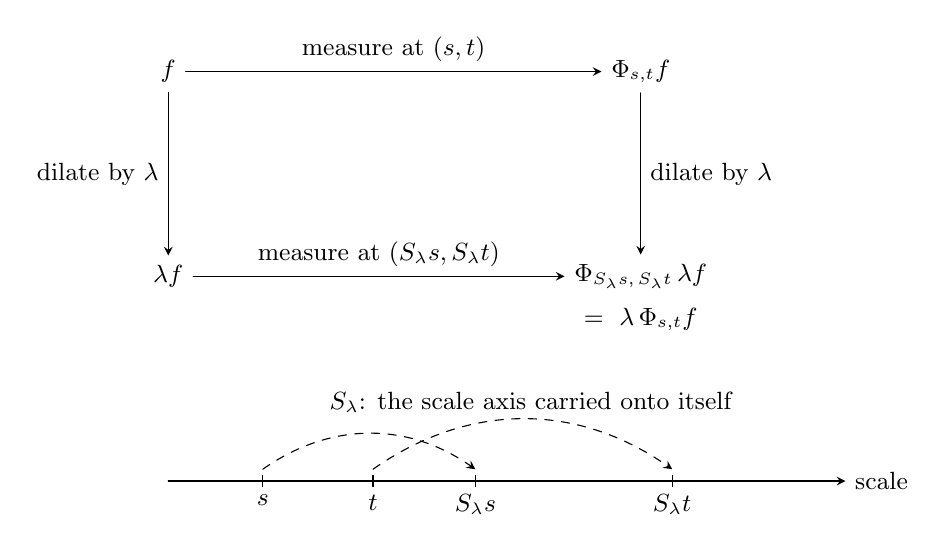
\begin{tikzpicture}[every node/.style={font=\small}, line cap=round, >=stealth]

% ---------- the commuting square ----------
\node (f)   at (0,2.6)   {$f$};
\node (Pf)  at (6.0,2.6) {$\Phi_{s,t} f$};
\node (Df)  at (0,0)     {$\Dil{\lambda} f$};
\node (PDf) at (6.0,0)   {$\Phi_{S_\lambda s,\,S_\lambda t}\,\Dil{\lambda} f$};
\node[anchor=north] at (PDf.south) {$=\ \Dil{\lambda}\,\Phi_{s,t} f$};

\draw[->] (f)  -- node[above] {measure at $(s,t)$} (Pf);
\draw[->] (f)  -- node[left]  {dilate by $\lambda$} (Df);
\draw[->] (Pf) -- node[right] {dilate by $\lambda$} (PDf);
\draw[->] (Df) -- node[above] {measure at $(S_\lambda s, S_\lambda t)$} (PDf);

% ---------- the scale axis, relabelled ----------
\begin{scope}[yshift=-2.6cm]
  \draw[->] (0,0) -- (8.6,0) node[right] {scale};
  \foreach \p/\l in {1.2/$s$, 2.6/$t$} {
    \draw (\p,0.07) -- (\p,-0.07); \node[below] at (\p,-0.05) {\l};
  }
  \foreach \p/\l in {3.9/$S_\lambda s$, 6.4/$S_\lambda t$} {
    \draw (\p,0.07) -- (\p,-0.07); \node[below] at (\p,-0.05) {\l};
  }
  \draw[->,dashed] (1.2,0.15) to[bend left=35] (3.9,0.15);
  \draw[->,dashed] (2.6,0.15) to[bend left=35] (6.4,0.15);
  \node[anchor=south] at (4.6,0.75) {$S_\lambda$: the scale axis carried onto itself};
\end{scope}

\end{tikzpicture}
\caption{Scale covariance (A8). Dilating the signal by $\lambda$ and then measuring is the
same as measuring and then dilating, provided the measurement is taken at the transported
scales $(S_\lambda s, S_\lambda t)$: the square commutes. The lower strip shows the
relabelling. Nothing ties the scale labels to a unit of length at this stage, so (A8) can
only ask that the family be mapped onto itself, with the labels rearranged by some
increasing bijection $S_\lambda$. \S\ref{sec:covariance} shows that the axioms determine
$S_\lambda$ and thereby a canonical parametrization of the scale axis.}
\label{fig:covariance-square}
\end{figure}


\subsection{The cascade property}\label{sec:axioms-cascade}

A record is itself a signal and can be measured further. A record at a coarser scale must
then be computable from the record at any finer scale, without returning to the raw
signal: a measurement of a measurement is a measurement, and the family closes under
composition,
\[
  \Phis{s}{t}\,\Phis{r}{s} \;=\; \Phis{r}{t}, \qquad r \le s \le t,
  \qquad\qquad \Phis{t}{t} = \mathrm{Id},
\]
which is (A6).

This is the axiom the paper changes. In \sscite{pauwels1995extended}, as throughout the
scale-space literature, the cascade is a one-parameter \emph{semigroup},
$K_sK_t = K_{s+t}$ in their notation, and this single equation asserts two things at once
(Figure~\ref{fig:cascade}). The first is the closure just motivated: composites of
measurements are measurements. The second is tacit: the composite depends only on the
total \emph{amount} of scale crossed. Equivalently, the elementary smoothing applied
between fine scales equals the one applied between coarse scales. The increments are
stationary in the scale parameter (the operators commute in either reading). Nothing in
the measurement picture supports the second assertion. A
stage that carries a fine record to a slightly coarser one and a stage that does the same
deep in the hierarchy act on different records, and there is no a priori reason the two
operations should coincide.

The hemigroup form (A6) keeps the first assertion and drops the second, and nothing else:
scale becomes an ordered interval structure rather than an additive quantity. Two
consequences follow immediately. The family must be indexed by pairs, since an increment
$\Phis{s}{t}$ is no longer determined by the difference $t - s$. And the scale axis
acquires a gauge freedom (any increasing reparametrization of $[0,\infty)$ yields the
same family relabelled), which is why (A8) was stated with the relabelling $S_\lambda$
left free. \S\ref{sec:covariance} resolves the second: covariance determines the gauge up
to normalization. And the semigroup case reappears when stationarity of the increments is
reimposed: Corollary~\ref{cor:semigroup-case} returns the symmetric stable family, the
positive part of the extended class.

\subsection{Continuity and nondegeneracy}\label{sec:axioms-continuity}

Measurements at nearby scales must be comparable: the record depends continuously on the
pair of scales, jointly, in the norm of $\Lone$ (A7). Together with the diagonal condition
$\Phis{t}{t} = \mathrm{Id}$, continuity is the extended point in its two-parameter form: as
$t \downarrow s$ the record at scale $t$ recovers the record at scale $s$.

Finally, the scale axis carries no idle stretches: strictly coarser means strictly more
smoothed, $\Phis{s}{t} \ne \mathrm{Id}$ for $s < t$ (ND). Nondegeneracy is a normalization
rather than a restriction. A family that stalls on an interval of scales is the same
family on a smaller scale axis.

\subsection{The axiom system}\label{sec:axioms-system}

% shared with blueprint def:cascade-family
\begin{definition}[symmetric cascade measurement family]\label{def:cascade-family}
A family of linear operators $\Phis{s}{t} : \Lone \to \Lone$, $0 \le s \le t < \infty$, is a
\emph{symmetric cascade measurement family} if:
\begin{enumerate}
\item[(A1)] \emph{Boundedness.} Each $\Phis{s}{t}$ is a bounded operator on $\Lone$.
\item[(A2)] \emph{Translation covariance.} $\Phis{s}{t}\,\Tr{a} = \Tr{a}\,\Phis{s}{t}$ for
every $a \in \RR$.
\item[(A3)] \emph{Reflection symmetry.} $\Phis{s}{t}\,R = R\,\Phis{s}{t}$.
\item[(A4)] \emph{Positivity.} $\Phis{s}{t}\,L^1_+ \subseteq L^1_+$.
\item[(A5)] \emph{Unit mass.} $\int \Phis{s}{t} f = \int f$ for every $f \in L^1_+$.
\item[(A6)] \emph{Cascade (hemigroup).} $\Phis{t}{t} = \mathrm{Id}$, and
$\Phis{s}{t}\,\Phis{r}{s} = \Phis{r}{t}$ for all $r \le s \le t$.
\item[(A7)] \emph{Continuity.} For every $f \in \Lone$ the map $(s,t) \mapsto \Phis{s}{t}f$ is
continuous from $\{0 \le s \le t\}$ to $\Lone$.
\item[(A8)] \emph{Scale covariance.} There is a family $(S_\lambda)_{\lambda > 0}$ of
increasing bijections of $[0,\infty)$ with
$\Dil{\lambda}\,\Phis{s}{t} = \Phi_{S_\lambda s,\,S_\lambda t}\,\Dil{\lambda}$ for all
$0 \le s \le t$ and all $\lambda > 0$.
\item[(ND)] \emph{Nondegeneracy.} $\Phis{s}{t} \ne \mathrm{Id}$ whenever $s < t$.
\end{enumerate}
\end{definition}

% blueprint rem:provenance-pauwels, copied; chapter references made section references
\begin{remark}[provenance: Pauwels et al.]\label{rem:provenance-pauwels}
The axioms of \sscite{pauwels1995extended} are, for a family $\{K_t\}_{t \ge 0}$: a linear
integral operator with an $\Lone$ kernel, shift invariance, evenness of the kernel, unit mass,
continuity of the kernel in $x$ and in $t$, \emph{recursivity} $K_sK_t = K_{s+t}$, and scale
invariance with a free rescaling function, $k_t(x) = \psi(t)^{-1}\phi(x/\psi(t))$ with $\psi$
continuous, strictly increasing, $\psi(0) = 0$ and $\psi(t) \to \infty$. Their linearity,
integral form and shift invariance are (A1)--(A2) together with the representation of
\S\ref{sec:representation}. Evenness is (A3), unit mass is (A5), and continuity in $t$ is
(A7). Recursivity is (A6) with the tacit assumption that the increments are stationary in
the scale parameter, which is what this article drops. Their $\psi$ is the relabelling $S_\lambda$ of (A8), recovered
rather than posited in Proposition~\ref{prop:canonical-gauge}. Two things they assume and
this article does not: kernels that are continuous \emph{functions}, and the semigroup.
Measures are allowed here so that the identity is the diagonal limit, and nothing is lost,
since by Proposition~\ref{prop:kernel-regularity} every nondegenerate admissible kernel has
a density anyway. Positivity, which in their paper enters only at the end, to bound the
stability index through a second moment, is an axiom here.
\end{remark}

\subsection{Two members}\label{sec:axioms-members}

Two members are checked before the general theory is developed: the Gaussian family,
with no jumps, and a family with jumps of every size and every moment finite. The axioms are
checked on both, for the Gaussian family directly and for the second member through the
exponents of its increments, which uses the admissibility criterion of the general theory
(Figure~\ref{fig:members}).

% shared with blueprint prop:two-members
\begin{proposition}[two members]\label{prop:two-members}
\begin{enumerate}
\item \emph{(The Gaussian family.)} Let $g_v$ be the centred Gaussian law of variance $v$, so
that $\hat g_v(\omega) = e^{-v\omega^2/2}$, and put $\Phis{s}{t}f := g_{t^2-s^2} * f$ for
$0 \le s \le t$. This family satisfies (A1)--(A8) and (ND), with $S_\lambda t = \lambda t$.
\item \emph{(The \Matern{} family.)} For $\gamma > 0$ let $\rho_{s,t}$ be the symmetric
probability measure with
\[
  \hat\rho_{s,t}(\omega) = \Bigl(\frac{1 + s^2\omega^2}{1 + t^2\omega^2}\Bigr)^{\gamma},
  \qquad 0 \le s \le t,
\]
and put $\Phis{s}{t}f := \rho_{s,t} * f$. This family satisfies (A1)--(A8) and (ND), with
$S_\lambda t = \lambda t$. Its kernel at scale $t$ has mean displacement $0$, variance
$2\gamma t^2$, and every moment finite.
\end{enumerate}
\end{proposition}

The Gaussian clause is elementary at the kernel: variances add, which is (A6); the image of
$g_v$ under $x \mapsto \lambda x$ is $g_{\lambda^2v}$, which is (A8); and $g_v$ being a
symmetric probability density gives (A1)--(A5). The Mat\'ern clause is elementary in the
same way once its kernels are known to be symmetric probability measures, which is the one
non-obvious point: the exponent $\gamma\log(1 + \omega^2)$ is admissible, with the profile
$2\gamma e^{-x}$, by Proposition~\ref{prop:matern-exponent} in the appendix. Two clauses are
not elementary at the kernel and are proved at the operator, as the proof shows: (A7), which
asks for strong convergence in $\Lone$ and not merely weak convergence of the kernels, and
(ND), which asks that the operator is not the identity and not merely that the transform is
not $1$. Both members are machine-checked in full, every axiom including (A7), and so is
the moment clause of (2), on Lean core: the mean and the variance directly, and the
finiteness of every moment through the Gaussian-mixture route of
Proposition~\ref{prop:matern-exponent}(3). The kernel itself is known in closed form, and
the proposition does not state it: it is the symmetric variance-gamma density, cited
(\sscite{fischer2025variance}, the density (1.1) and the characteristic function (2.12)),
which for $\gamma > \tfrac12$ is the Mat\'ern kernel of smoothness $\gamma - \tfrac12$ and
range $t$ (the smoothness index governs the behaviour at the origin, the range is the
length unit of the exponential tail; for $\gamma \le \tfrac12$ the kernel is unbounded at
the origin and is a density but not a covariance function). Nothing in this paper uses the
closed form.

\begin{proof}
(1) Each $g_v$ with $v > 0$ is a symmetric probability density, and $g_0 := \delta_0$; so
(A1)--(A5) hold by the converse clause of Lemma~\ref{lem:convolution-representation}, (A3)
because $g_v$ is invariant under reflection. For (A6),
$\hat g_{t^2-s^2}\,\hat g_{s^2-r^2} = \hat g_{t^2-r^2}$ and transforms determine measures
(Proposition~\ref{prop:fourier-uniqueness}); $\Phis{t}{t} = \mathrm{Id}$ is $g_0 = \delta_0$.
For (A8) with $S_\lambda t = \lambda t$, the image of $g_v$ under $x \mapsto \lambda x$ is
$g_{\lambda^2 v}$, and $\lambda^2(t^2 - s^2) = (\lambda t)^2 - (\lambda s)^2$. For (ND): a
probability measure whose convolution operator fixes every $f \in \Lone$ is $\delta_0$ ---
convolve a bump attaining a strict maximum at the origin, and read the resulting identity
there --- and $g_{t^2-s^2} = \delta_0$ only when $s = t$.

For (A7) the semigroup does the work. For $0 \le v \le w$ one has $g_w = g_v * g_{w-v}$, so
$g_w * f - g_v * f = g_v * (g_{w-v} * f - f)$, and convolution by a probability measure is a
contraction of $\Lone$:
\[
  \| g_w * f - g_v * f \|_1 \ \le\ \| g_{w-v} * f - f \|_1 .
\]
Continuity in $(s,t)$ therefore reduces to continuity of $v \mapsto g_v * f$ at $v = 0$, and that
follows from the elementary estimate
\[
  \| \mu * f - f \|_1 \ \le\ \int_\RR \Theta_f(y)\, \mu(dy),
  \qquad \Theta_f(y) := \| \Tr{y} f - f \|_1,
\]
valid for every probability measure $\mu$, which is Fubini applied to
$(\mu * f - f)(x) = \int (f(x-y) - f(x))\,\mu(dy)$. The function $\Theta_f$ is continuous,
bounded by $2\|f\|_1$, and vanishes at $y = 0$, by strong continuity of translation on $\Lone$;
and $g_v$ is the image of $g_1$ under $z \mapsto \sqrt{v}\,z$, so
$\int \Theta_f\,dg_v = \int \Theta_f(\sqrt{v}\,z)\,g_1(dz) \to 0$ as $v \to 0$ by dominated
convergence.

(2) By Proposition~\ref{prop:matern-exponent} the function
$F(\omega) = \gamma\log(1 + \omega^2)$ is admissible in the sense of
Theorem~\ref{thm:main-characterization}, with Gaussian coefficient $0$ and folded profile
$k(x) = 2\gamma e^{-x}$, and $\hat\rho_{s,t}(\omega) = \exp[-(F(t\omega) - F(s\omega))]$; so
$\rho_{s,t}$ is the increment kernel of the admissible family attached to $F$ in the
canonical gauge. That the kernel at scale $t$ is the Mat\'ern kernel of smoothness
$\gamma - \tfrac12$ and range $t$ is the Fourier pair of the symmetric variance-gamma law
(\sscite{fischer2025variance}, (1.1) and (2.12)), cited; the variance and the finiteness of
every moment are Proposition~\ref{prop:matern-exponent}(3).

The axioms themselves are read off the transform and need neither of those. (A1)--(A5) are
again Lemma~\ref{lem:convolution-representation}, the kernels being symmetric probability
measures; (A6) is $\hat\rho_{r,s}\,\hat\rho_{s,t} = \hat\rho_{r,t}$ together with
$\hat\rho_{t,t} \equiv 1$ and Proposition~\ref{prop:fourier-uniqueness}; (A8) with
$S_\lambda t = \lambda t$ is $\hat\rho_{s,t}(\lambda\omega) = \hat\rho_{\lambda s,\,\lambda t}(\omega)$;
and (ND) is $\hat\rho_{s,t}(1) = \bigl((1+s^2)/(1+t^2)\bigr)^{\gamma} < 1$ for $s < t$.

(A7) costs more than in (1), because a hemigroup has no single increment parameter:
$\Phis{s}{t}$ and $\Phi_{s',t'}$ are compared through the intermediate $\Phi_{s',t}$, one
endpoint at a time. Moving the left endpoint leaves an increment applied \emph{first}, which
the contraction bound absorbs as in (1); moving the right endpoint leaves one applied
\emph{last}, to $\Phi_{s',t}f$ rather than to $f$, so the estimate above is read at that
element --- which loses nothing, since translation commutes with convolution and hence
$\Theta_{\mu * f} \le \Theta_f$. Both remainders are increments whose two endpoints come
together, and for those $\hat\rho_{a,b} \to 1$ pointwise, so $\rho_{a,b} \to \delta_0$ weakly
(Proposition~\ref{prop:levy-continuity}) and $\int \Theta_f\,d\rho_{a,b} \to \Theta_f(0) = 0$.
On the diagonal $s = t$ the intermediate is unavailable and unnecessary: the limit operator
is the identity, and one collapsing increment suffices.

Both families are verified in the machine-checked development, every axiom including (A7);
the appeal to Proposition~\ref{prop:matern-exponent} carries the \emph{existence} of the
Mat\'ern kernels, and the cited closed form is not used in the verification of the axioms.
\end{proof}

The Gaussian family is the member with no jumps, its profile being zero, and it is an
extreme ray of the cone of admissible exponents (Remark~\ref{rem:gaussian-extreme}). The
Mat\'ern family has jumps of every size. Theorem~\ref{thm:main-characterization}
characterizes all families satisfying the axioms.

% Figure: the two members of §3, the Gaussian and the Matern family, at unit canonical scale.
% Referenced from §3.6 after prop:two-members. Generated by scripts/make-fig-members.py from the
% transforms alone (numerical Fourier inversion of (1 + omega^2)^{-gamma}; no Bessel function),
% so the picture rests on prop:two-members' transform and on nothing cited. The tail statements
% in the caption are what the computed curves show, not theorems of this paper.
\begin{figure}[t]
\centering

\includegraphics[width=\textwidth]{fig-members.png}
\caption{The two members of Proposition~\ref{prop:two-members} at unit canonical scale,
computed from their transforms. Left, linear scale: the variance-gamma densities with
transform $(1 + \omega^2)^{-\gamma}$ for $\gamma = \tfrac12, 1, 2, 4$, and a Gaussian of
variance $4$, the variance the $\gamma = 2$ member has by
Proposition~\ref{prop:matern-exponent}(3); the variances of the four densities differ,
$2\gamma$ each. At $\gamma = \tfrac12$ the density is unbounded at the origin and the curve is
clipped; at $\gamma = 1$ it is the Laplace density $e^{-|x|}/2$, with a cusp. Right, the same
curves on a logarithmic scale: the four densities fall off exponentially, the Gaussian as
$e^{-x^2/8}$.}
\label{fig:members}
\end{figure}


\subsection{Without positivity: an affine family through the Gaussian}\label{sec:axioms-nopositivity}

In the semigroup theory positivity only trims the class. The next proposition shows that
under the hemigroup it decides whether a classification exists at all: without (A4) the
hemigroup axioms admit an
infinite-dimensional affine family of exponents through the Gaussian, of which exactly the
members of the form \ref{eq:sd-profile} are positive, so no classification in the style of
Theorem~\ref{thm:main-characterization} is possible without (A4). No attempt is made to
describe the non-positive class beyond this.

% shared with blueprint prop:no-positivity-no-classification
\begin{proposition}[without positivity: an affine family through the Gaussian]
\label{prop:no-positivity-no-classification}
Let $A(\RR) := \{\hat h : h \in \Lone\}$ be the Wiener algebra and let $\phi \in A(\RR)$ be
real and even with $\phi(0) = 0$. Put $F(\omega) := \omega^2 + \phi(\omega)$ and define
$\mu_{s,t}$, $0 \le s \le t$, by $\hat\mu_{s,t}(\omega) = e^{-(F(t\omega) - F(s\omega))}$. Then
each $\mu_{s,t}$ is a finite symmetric signed measure, an integrable function when $s < t$, and
$\Phis{s}{t} := \mu_{s,t} * {}$ satisfies (A1)--(A3), (A5)--(A8) with
$S_\lambda t = \lambda t$, and (ND). It satisfies (A4) if and only if $F$ is of the form
\ref{eq:sd-profile}. In particular, for $q \in \Lone$ even, supported in $\{|x| \ge 1\}$, of
mean zero and not almost everywhere nonnegative, and
$\phi_\varepsilon(\omega) := \varepsilon\int_\RR (1 - \cos\omega x)\,q(x)\,dx$, the family
violates (A4) for every $\varepsilon \ne 0$.
\end{proposition}

Every step is elementary, and two of the three clauses are machine-checked: the positivity
equivalence, forwards by reading (A4) at an approximate identity and backwards by
identifying the constructed law through the Jordan decomposition of the signed kernel into
its positive and negative parts, and the final sentence, that the family built from $q$
violates (A4) for every $\varepsilon \ne 0$. What is not machine-checked is the first
clause, the construction of $h_{s,t}$ in the Wiener algebra $A(\RR)$ of transforms of
integrable functions and the verification of the axioms for the signed family: the library
used carries the $\Lone$
Fourier transform but not $A(\RR)$ as a Banach algebra, and a route through the
convolution operators in place of the functions has been estimated and not carried out. That
clause rests on the printed proof alone.

\begin{proof}
\emph{The family.} $A(\RR)$ is a Banach algebra under pointwise multiplication, invariant
under dilation, so $\phi_{s,t} := \phi(t\,\cdot) - \phi(s\,\cdot)$ lies in it, and
$e^{-\phi_{s,t}} = 1 + \hat h_{s,t}$ with $h_{s,t} \in \Lone$, the exponential series converging
in the algebra. (The map $b \mapsto \phi(b\,\cdot)$ is \emph{not} norm-continuous into $A(\RR)$
at $b = 0$: for $b > 0$ it is the transform of the dilate $h_b := b^{-1}h(\cdot/b)$, of norm
$\|h\|_1$, while $\phi(0\,\cdot) = \phi(0) = 0$. So $h_{s,t}$ is not norm-continuous up to the
edge $s = 0$, and (A7) is argued below through operators.) With $g_{2(t^2-s^2)}$ the
Gaussian kernel of variance $2(t^2-s^2)$, whose transform is $e^{-(t^2-s^2)\omega^2}$ in the
normalization $\hat g_v = e^{-v\omega^2/2}$ of Proposition~\ref{prop:two-members} --- a
density for $s < t$, and $\delta_0$ on the diagonal --- we get
$\mu_{s,t} = g_{2(t^2-s^2)} + g_{2(t^2-s^2)} * h_{s,t}$: a finite signed measure,
symmetric because its transform is real and even, and an integrable function for $s < t$.

\emph{The axioms.} (A1) holds with $\|\mu_{s,t}\| \le 1 + \|h_{s,t}\|_1$; (A2) because
convolution commutes with translation; (A3) by symmetry; (A5) from $\hat\mu_{s,t}(0) = 1$; (A6)
because the exponents add and transforms determine measures
(Proposition~\ref{prop:fourier-uniqueness}); (A8) with $S_\lambda t = \lambda t$, because
$F(\lambda t\omega) - F(\lambda s\omega)$ is $F(t\,\cdot) - F(s\,\cdot)$ evaluated at
$\lambda\omega$; and (ND) because
$F(t\omega) - F(s\omega) = (t^2-s^2)\omega^2 + \phi_{s,t}(\omega)$ is unbounded, $\phi_{s,t}$
being bounded. For (A7), let $h_e$ be the even part of $h$ and $H_b f := h_b * f$ for
$b > 0$, with $h_b$ the dilate of $h_e$, and $H_0 := 0$. Each $H_b$ is a bounded operator on
$\Lone$ of norm at most $\|h\|_1$, the $H_b$ commute with one another and with the Gaussian
convolutions, and $b \mapsto H_b f$ is continuous on $[0,\infty)$ for every $f \in \Lone$: at
$b > 0$ by strong continuity of dilation, and at $b = 0$ because $h_b$ is an approximate
identity of total mass $\int h_e = \phi(0) = 0$, so $h_b * f \to 0$ in $\Lone$. Then
$\mu_{s,t} * f = g_{2(t^2-s^2)} * \exp\bigl(-(H_t - H_s)\bigr)f$, the exponential series converging in
operator norm uniformly in $(s,t)$, its $n$-th term being bounded by $(2\|h\|_1)^n/n!$. A product
of uniformly bounded, strongly continuous operator families is strongly continuous, so each
partial sum is, hence so is the sum, and composing with the strongly continuous Gaussian family
gives (A7). The route is strong continuity throughout, and it does not need $h_{s,t}$ to depend
continuously on $(s,t)$ in norm, which it does not at $s = 0$.

\emph{Positivity.} Suppose (A4) holds. The kernels $\mu_{s,t}$ are so far only integrable
functions, and Theorem~\ref{thm:main-characterization} is a statement about probability
kernels, so the first step is to see that (A4) makes them nonnegative. Convolve with an
approximate identity: $\mu_{s,t} * \rho_\varepsilon \ge 0$ for every $\varepsilon > 0$ because
$\rho_\varepsilon \ge 0$, and $\mu_{s,t} * \rho_\varepsilon \to \mu_{s,t}$ in $\Lone$; the
positive cone of $\Lone$ is closed, so $\mu_{s,t} \ge 0$ almost everywhere. Its total mass is
$\hat\mu_{s,t}(0) = 1$, so $\mu_{s,t}\,dx$ is a probability measure, the family satisfies
every axiom, and Theorem~\ref{thm:main-characterization} applies. It returns a gauge $\chi$
and a profile $P$ with $F(t\omega) - F(0) = P(\chi(t)\omega)$; reading that at $t = 1$ and
using $F(0) = \phi(0) = 0$ gives $F(\omega) = P(\chi(1)\omega)$, and $\chi(1) > 0$, so $F$ is
$P$ dilated and is itself of the form \ref{eq:sd-profile}.

Conversely, suppose $F$ has that form. Each increment exponent
$\omega \mapsto F(t\omega) - F(s\omega)$ is then a member of $\NDs$ by
Lemma~\ref{lem:selfdecomposable-exponents}, hence the exponent of a symmetric probability
law $\nu$ (Proposition~\ref{prop:fourier-toolbox}); and $\nu$ has the same cosine transform
as $\mu_{s,t}$, which is even and integrable. The Jordan parts of $\mu_{s,t}$ split it as a
difference of two finite measures whose characteristic functions are determined by that
cosine transform, evenness making both sine transforms vanish, so
$\mu_{s,t}^+\,dx = \nu + \mu_{s,t}^-\,dx$ by Proposition~\ref{prop:fourier-uniqueness}.
Testing this on the set where $\mu_{s,t}$ is negative makes its left side vanish, so
$\mu_{s,t}^- = 0$ almost everywhere: $\mu_{s,t} \ge 0$, and (A4) is positivity of an
integral.

\emph{The example.} Write $g(\omega) := \int (1 - \cos\omega x)\,q(x)\,dx$, so that
$F = \omega^2 + \varepsilon g$. Since $\int q = 0$ we have $g = -\hat q$, so $g$ is bounded and
$g(0) = 0$; hence $\phi_\varepsilon = -\varepsilon\,\hat q$ lies in $A(\RR)$, real and even
because $q$ is, and the family is one of those described. (Mean zero is not cosmetic: without
it $\phi_\varepsilon$ tends to $\varepsilon\int q \ne 0$ at infinity, which no member of the
Wiener algebra does.)

Suppose $F$ were of the form \ref{eq:sd-profile}, with Gaussian coefficient $a \ge 0$ and
\Levy{} measure $\nu$ on $(0,\infty)$ subject to $\int (1 \wedge x^2)\,\nu(dx) < \infty$.
Average the two readings of $F$ over $[0,T]$. The elementary primitive
$\int_0^T (1 - \cos\omega x)\,d\omega = T\bigl(1 - \frac{\sin Tx}{Tx}\bigr)$ and Tonelli give,
for every $T > 0$,
\[
  \frac{T^2}{3}
   + \varepsilon\int \Bigl(1 - \frac{\sin Tx}{Tx}\Bigr) q(x)\,dx
  \;=\; \frac{a\,T^2}{3}
   + \int \Bigl(1 - \frac{\sin Tx}{Tx}\Bigr) \nu(dx),
\]
both integrals converging absolutely because
$0 \le 1 - \frac{\sin u}{u} \le \min(2,\, u^2/6)$.

Read this identity at rate $T^2$. Divided by $T^2$, the perturbation term vanishes in the limit
because its integral is bounded by $2\|q\|_1$, and the \Levy{} term vanishes by dominated
convergence, the integrand $T^{-2}\bigl(1 - \frac{\sin Tx}{Tx}\bigr)$ being at most
$2\,(1 \wedge x^2)$ for $T \ge 1$ and tending to $0$ pointwise. Hence $a = 1$, and the identity
reduces to
$\int \bigl(1 - \frac{\sin Tx}{Tx}\bigr)\nu(dx)
 = \varepsilon\int \bigl(1 - \frac{\sin Tx}{Tx}\bigr) q(x)\,dx$.

Now read it at rate $1$. The right-hand side tends to $\varepsilon \int q = 0$ as
$T \to \infty$, by dominated convergence against $|q|$. On the left,
$1 - \frac{\sin Tx}{Tx} \to 1$ at every $x \ne 0$ and $\nu$ gives the origin no mass, so Fatou
forces $\nu\bigl((0,\infty)\bigr) = 0$. With $a = 1$ and $\nu = 0$, \ref{eq:sd-profile} reads
$F(\omega) = \omega^2$, that is $\varepsilon\,g \equiv 0$, that is $\hat q \equiv 0$ because
$\varepsilon \ne 0$. An even integrable function whose cosine transform vanishes identically is
null: its positive and negative parts are two finite measures whose cosine transforms agree and
whose sine transforms both vanish, evenness being what kills the latter, so
Proposition~\ref{prop:fourier-uniqueness} identifies them. Thus $q = 0$ almost everywhere,
against the hypothesis that $q$ is not almost everywhere nonnegative --- and both signs of
$\varepsilon$ are covered, neither the identity nor either reading of it seeing the sign. So
$F$ is not of the form \ref{eq:sd-profile}, and (A4) fails by the previous paragraph.
\end{proof}

% blueprint rem:signed-levy-uniqueness, copied
\begin{remark}[the route through signed uniqueness]\label{rem:signed-levy-uniqueness}
The last clause of the proposition, that the family built from $q$ violates (A4), is usually
argued the other way round: $\omega^2 + \phi_\varepsilon$ \emph{is} a
signed \Levy--Khintchine representation, with Gaussian coefficient $1$ and signed measure
$\varepsilon\,q(x)\,dx$, and such representations are unique among signed measures $m$ with
$\int (1 \wedge x^2)\,|m|(dx) < \infty$. Since $\varepsilon\,q$ is not a nonnegative measure,
$F$ is not of the form \ref{eq:sd-profile}. The uniqueness is the averaging identity
\[
  \frac{1}{2h}\int_{\omega-h}^{\omega+h}\psi(u)\,du \;-\; \psi(\omega)
  \;=\; \frac{a\,h^2}{3}
   + \int \cos(\omega x)\Bigl(1 - \frac{\sin hx}{hx}\Bigr)\,m(dx)
\]
for $\psi(\omega) = a\omega^2 + \int (1-\cos\omega x)\,m(dx)$, whose right-hand side is a
constant plus the Fourier--Stieltjes transform of the finite signed measure
$\bigl(1 - \frac{\sin hx}{hx}\bigr)\,m(dx)$; so $\psi$ determines that measure for every
$h > 0$, hence $m$ off the origin, hence $a$. This is the more informative statement, because
it is about the representation rather than about one $F$. It is
also strictly more than the proposition needs, and it is \textbf{not machine-checked}: the
proof of record above replaces it by the two readings of the averaged identity, at the
rates $T^2$ and $1$, which identify $a$ and $\nu$
for the single exponent at hand and never mention a signed measure.
\end{remark}

Under recursivity the same setting forces $F(\omega) = a|\omega|^\alpha$ with $\alpha > 0$: a
one-parameter class whether or not positivity is imposed, positivity entering only to bound
$\alpha \le 2$ (\sscite{pauwels1995extended}, Prop.~1). Under the hemigroup, dropping
positivity admits the affine family $\omega^2 + A(\RR)_{\mathrm{even},0}$ through the
Gaussian, and the same family through every admissible exponent unbounded at infinity. The
positive members of the first are exactly those of the form \ref{eq:sd-profile}, and the
others have no description in the form of the theorem.

% blueprint rem:provenance-causal, copied; this section's relation-to-the-causal-theory remark,
% placed at the section's end (the external review, D2, 2026-09-14) and shortened
\begin{remark}[relation to the causal theory]\label{rem:provenance-causal}
(A1), (A2), (A4)--(A8) and (ND) are the axioms of the time-causal article
\sscite{fagerstrom2026hemigroup} up to the change of letters, and (A3) replaces causality
by reflection symmetry: the axiom that removed the Gaussian there is the axiom that admits
it here. Three consequences are visible already. The convolution representation yields
symmetric probability measures on $\RR$ rather than probability measures on a half-line,
and the Fourier transform can vanish where the Laplace transform cannot, so a nonvanishing
lemma (Lemma~\ref{lem:nonvanishing}) replaces the positivity of the causal integrand. The
drift slot of the causal profile representation is occupied here by the Gaussian
coefficient, so the member that stands where the pure delay stood is the Gaussian scale
space itself, admissible, extreme and nondegenerate. And the gauge argument, which used the
causal vanishing lemma twice, is re-routed through a smoothed transform
(Corollary~\ref{cor:smoothed-transmittance}) and a dilation argument
(Lemma~\ref{lem:dilation-atom}), the exclusion of lattice laws following from covariance
(Lemma~\ref{lem:no-lattice}) rather than from the function class.
\end{remark}
